\chapter{Methodology Part 2: Advancing Several Layers}

In the previous chapter, we talked about how the very first layer of the mesh is generated. Starting from the discussion of extruding one boundary vertex onto the sub-surface, we went on explained how all the vertices on the boundary curve of the sub-surface are extruded and subsequently, how the advancing front is recovered so as to move on to the next layer. We also talked about how extrusion length scaling at concave corners helps us avoid immediate front collapse and improves overall mesh quality. In this chapter, we are going to discuss some of the important subroutines which help complete the anisotropic surface mesh.

We will start by discussing the subroutine used to control the aspect ratio as we advance several layers in the mesh. Combining triangular mesh elements to quad elements would be discussed next. Subsequently, mesh smoothing and collision handling would be discussed.

\section{Aspect Ratio Control and Sub-surface Interior Improvement}

\subsection{Vertex Decimation on the Front}
\label{aspectRatioControl}

As the advancing front moves into the surface interior, the layers grow in size. This is done for the purpose of giving a higher refinement at the boundary curves. As the size of the layer grows, the aspect ratio of the mesh elements generated decrease. Also, some of the vertices on the front might come so close to each other that the aspect ratio approaches unity. Growing the layers further with all the vertices on the front would lead to anisotropy in the orthogonal direction  and/or front overlap. Hence, decimation of some of the front vertices is necessary to proceed with the next few layers.

\begin{figure}[hbt!]
\centering
\begin{subfigure}{.5\textwidth}
  \centering
  \includegraphics[width=.9\linewidth]{img/m2/edge-collapse/collapse1.eps}
  \caption{}
  \label{collapse1}
\end{subfigure}%
\begin{subfigure}{.5\textwidth}
  \centering
  \includegraphics[width=.9\linewidth]{img/m2/edge-collapse/collapse2.eps}
  \caption{}
  \label{collapse2}
\end{subfigure}
\begin{subfigure}{.5\textwidth}
  \centering
  \includegraphics[width=.9\linewidth]{img/m2/edge-collapse/collapse3.eps}
  \caption{}
  \label{collapse3}
\end{subfigure}
\caption{Edge collapse on an advancing front to avoid encroachment of points. In (a), two points in the kid layer $P_1$ and $P_2$ are sufficiently close to each other. Their parent layer is highlighted. If both the points advance to the next layer, then the next front would fail to recover. Hence, the edge between them is chosen to collapse. (b) shows the result of the edge collapse. The new location of both the points is the average position of their initial location. (c) shows how the next front looks like.}
\label{edge-collapse}
\end{figure}

Once we have recovered the advancing front by iterative edge swaps to connect the kid points in the mesh, we check for vertices on the front that are too close to each other relative to the extrusion length. For instance, vertices which are near a concave corner could encroach each other if they are not decimated. Another example of a situation where vertex decimation on the advancing front becomes necessary is when the front has advanced to a substantial distance from the surface boundaries. In such a case, the extrusion length on the front has grown so much that the aspect ratio approaches unity. Decimating vertices from the front which are at a substantial distance from surface boundaries helps prevent the cell aspect ratio, ie front edge length over extrusion length, from dropping below one.

To check for vertices to decimate, we iterate through the vertices in the front and identify the ones which are too close to their neighbours. Vertex decimation is done through the edge-collapse routine as described in \cite{hoppe1994mesh}. The threshold edge length between two points on the front is set to be $2 \tan(\pi/8)$ times the average extrusion length at those points. This value is set so as to minimize the normalized maximum deviation of angle from $90^\circ$ for quad elements. Hence, the threshold ensures that the anisotropic properties are retained for several layers into the surface. All short edges on the front are collapsed using the edge-collapse algorithm. An example of an edge-collapse on the front is shown in Figure \ref{edge-collapse}. Here, two points $P_1$ and $P_2$ are collapsed into a single point which forms a part of the next front on the surface. Mathematically,

\begin{equation}
l_{\mathit{collapse}} = 2 \cdot \; tan \left( \frac{pi}{8} \right) \cdot \; x_n \; ;
\end{equation}

where $l_{\mathit{collapse}}$ is the minimum length of an edge on the advancing front which will not be considered for edge collapse and $x_n$ is the extrusion length at the $n^{th}$ layer.

%Validation checks are made before collapsing an edge. The deviation of the triangles formed as a result of edge collapse from the underlying surface is constrained to be less than $30^{\circ}$ to limit the deviation of the mesh from the ground truth surface $S$. 

Topological and geometrical checks are done before an edge can be collapsed in the mesh. These include a threshold for the ratio of area of generated triangles and a limit on the dihedral angle between the adjacent triangles created by the collapse. The area threshold is set to be $10^8$. Also, edge-collapse is successful only if the triangles resulting from it are be within a limit of $\theta < 30^{\circ}$ from the surface(see Figure \ref{deviation-surface}). The threshold for the maximum dihedral angle between any two adjacent triangles that result from the edge-collapse is set to $40^{\circ}$. 

After we have a recovered the front and decimated encroaching vertices in the surface interior as well as on the advancing front through edge collapse, we queue up the immediate interior edges of the surface and swap them for maximizing mesh quality. This step is included so that we have a good interior triangulation at each step of the advancing layer routine. This step ensures that we do not have bad triangles causing problems as we continue to march.

The edge collapse subroutine on the advancing front helps in controlling the aspect ratio at the front and limit its minimum value to 1. Once the aspect ratio has approached a value of $1$ on the front, layers will continue to extrude without growth in their size. Additionally, at concave corners with low aspect ratios, the edge collapse subroutine helps in maintaining a valid front to continue marching towards surface interior.

\subsection{Vertex Decimation in Sub-Surface Interior}

As discussed in the previous chapter, we follow a closed advancing front methodology to generate the anisotropic surface mesh. The input triangulation $T$, which is the encoding of the surface $S$ is taken to be the initial mesh. Such a technique helps us in maintaining a complete and valid surface mesh at each step in the mesh generation process. However, this means that we need to do some additional work in deleting the vertices on the sub-surface imported initially which are no longer required to be a part of the anisotropic surface mesh. Fortunately, we have all the connectivity information of the vertices on the front. This means that we do not have to scan the 3D space near the vertex to find the encroaching points. Checking the vertices in surface interior which share an edge with the front vertex is sufficient.

\begin{figure}[hbt!]
\centering
\begin{subfigure}{.5\textwidth}
  \centering
  \includegraphics[width=.9\linewidth, trim={0 5cm 0  0}, clip]{img/m2/interior-vert-collapse/cc1.eps}
  \caption{}
  \label{cc1}
\end{subfigure}%
\begin{subfigure}{.5\textwidth}
  \centering
  \includegraphics[width=.9\linewidth, trim={0 5cm 0  0}, clip]{img/m2/interior-vert-collapse/cc2.eps}
  \caption{}
  \label{cc2}
\end{subfigure}
\begin{subfigure}{.5\textwidth}
  \centering
  \includegraphics[width=.9\linewidth, trim={0 5cm 0  0}, clip]{img/m2/interior-vert-collapse/cc3.eps}
  \caption{}
  \label{cc3}
\end{subfigure}%
\begin{subfigure}{.5\textwidth}
  \centering
  \includegraphics[width=.9\linewidth, trim={0 5cm 0  0}, clip]{img/m2/interior-vert-collapse/cc4.eps}
  \caption{}
  \label{cc4}
\end{subfigure}
\caption{Interior vertex decimation through edge collapse. The highlighted white line shows the advancing front. In (a), vertex $P_2$ is about to encroach the front. Hence, the best vertex for collapse is chosen among its neighbours. The best vertex for edge collapse here is $P_1$. Hence, $P_2$ is collapsed on to $P_1$. The connectivity after the edge collapse is shown in (b) where vertex $P$ represents the collapsed vertex. Similarly, in (c), vertex $P_2$ is about to encroach the advancing front and is collapsed onto vertex $P_1$ which is on the advancing front itself. The new connectivity is shown in (d) where all the possibly encroaching vertices for the advancing layer are decimated.}
\label{interior-vert-collapse}
\end{figure}

In other words, as the advancing front marches into the surface, vertices in the interior of the surface immediately next to the front are decimated to make way for the advancing layers. Before extruding a point $P$ on the advancing front, we check if any point in the surface interior with which it shares an edge agrees with the following condition. If it does, we decimate the interior vertex.

\begin{equation}
    d < max \left( \frac{l_{1}}{\sqrt{2}}, \, \frac{l_{2}}{\sqrt{2}}, \; c \cdot  \mathit{x_n}\right)
    \label{collapse-eq}
\end{equation}

Here $d$ is the distance between the point on the advancing front and the interior point, $l_1$ and $l_2$ are the lengths of adjacent front edges of the point on the front, c is a constant whose value is set as $2$ and $x_n$ is the extrusion length at the vertex on the $n^{th}$ front. This condition ensures decimation of vertices in the surface interior which are close to the advancing front and avoids any encroachment of surface interior vertices on the advancing layers. 

Validation checks for front edge collapse mentioned in the last subsection are also run during interior edge collapse. The quality criterion used for interior edge collapse is maximization of the minimum angle in the triangles thus produced. The best edge for collapse is chosen when decimating the interior vertices using this quality criterion. This is in contrast to the vertex decimation on the advancing front where the candidate edge for collapse is already identified. An illustrative example for surface interior vertex decimation can be seen in Figure \ref{interior-vert-collapse}.

\section{Combining Triangular Elements to Quadrilateral Elements}

In section \ref{sec-simplicial}, we discussed about the pros and cons of simplical and non-simplical mesh elements. Then, in section \ref{consolidate-motivation}, we talked about the motivation to produce a hybrid surface mesh which consists of both simplical and non-simplical mesh elements. Briefly, a hybrid anisotropic surface mesh which consists primarily of quadrilateral elements with a small number of triangular elements gives us the flexibility to mesh topologically complex surface geometries while keeping the average vertex connectivity of the mesh to a low value.

Almost all vertices in our closed advancing front method have a parent-kid relationship. The successor of a vertex is called its kid while the predecessor is called the parent. There are a couple of exceptions to this. First, vertices on the boundary curve do not have a parent as they are the zeroth layer of the mesh. Second, wherever an edge collapse operation is done, two kids from two different parent vertices collapse into a single vertex. This leaves a kid vertex with two parents, or, in other words, a two parents who share a common kid vertex.

\vspace{10pt}
\begin{figure}[hbt!]
\centering
\begin{subfigure}{\textwidth}
  \centering
  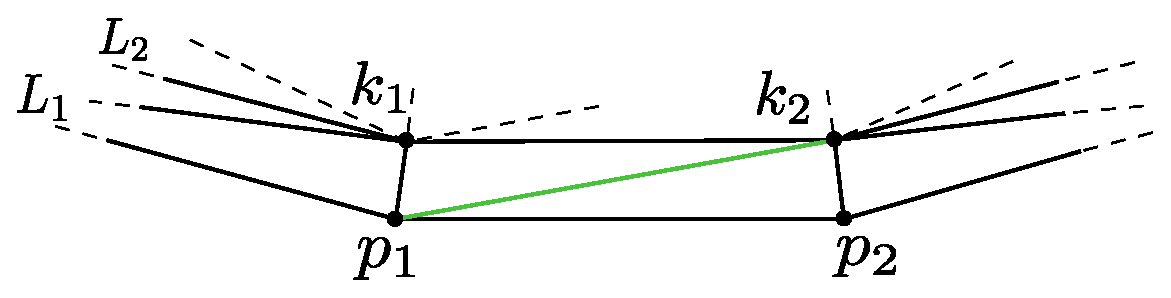
\includegraphics[width=.7\linewidth]{img/m2/combineTriToQuad.eps}
  \caption{}
  \label{triToQuad1}
\end{subfigure}
\begin{subfigure}{\textwidth}
  \centering
  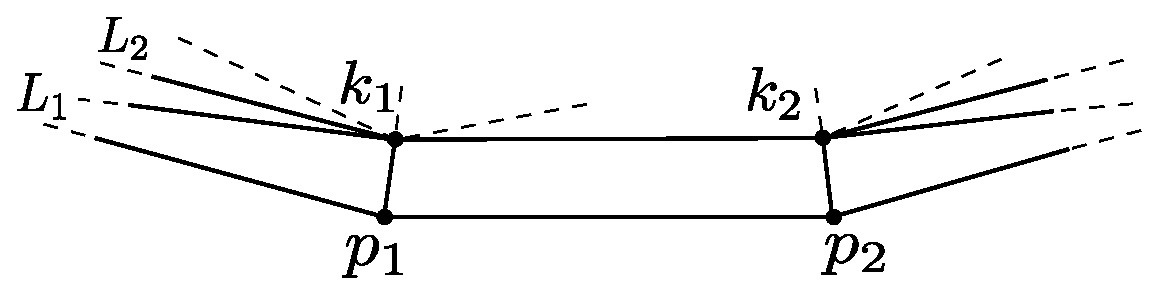
\includegraphics[width=.7\linewidth]{img/m2/combineTriToQuad2.eps}
  \caption{}
  \label{triToQuad2}
\end{subfigure}
\caption{}
\label{triToQuad}
\end{figure}

Apart from the two exceptions just mentioned, all the vertices have a parent and a kid. This gives some structure to our mesh. As the layers grow in the normal direction to the boundary curve, this helps us in generating rectangular quadrilateral elements easily. Edges are removed from the finished layers so as to generate superior quality quadrilateral cells. As the layers advance from the boundary curves towards the tangential direction onto the surface, the quadrilateral elements generated retain the boundary topology several layers into the interior of the surface. The quality of a quadrilateral element is calculated as the inverse of the maximum deviation of its interior angles from 90 degrees. This criterion is selected so as to prefer rectangular elements and retain the boundary representation on the surface mesh. Starting from the first layer generated on the surface, multiple iterations of this subroutine are run for the same layer to ensure as few triangular elements are left per layer as possible.

Consider Figure \ref{triToQuad1}. $L_1$ and $L_2$ denote two successive layers on the advancing layer mesh. Points $p_1$ and $p_2$ are on the parent layer $L_1$ and their kids, $k_1$ and $k_2$, respectively, are on the kid layer $L_2$. All the edges in the neighbourhood of $p_1$ and $p_2$ which are not on the advancing front are queued. Then, these edges are sorted in order of the quality of the quadrilateral elements generated after their removal. Finally, all the edges in the queue are deleted until both the elements which share the edge are triangular. The edged marked in green color in the figure is deleted in the process which results in the deletion of two triangular elements and generation of a new quadrilateral element. The local mesh after edge removal is shown in Figure \ref{triToQuad2}.

\vspace{10pt}
\begin{figure}[hbt!]
  \centering
  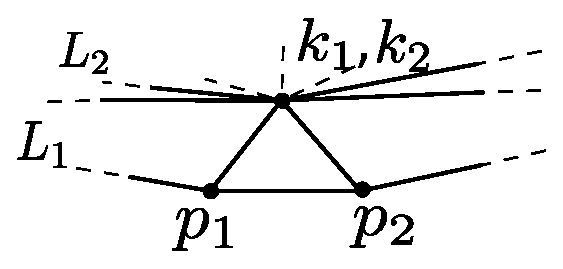
\includegraphics[width=0.5\linewidth]{img/m2/combineTriToQuad3.eps}
  \caption{•}
  \label{triLeft}
\end{figure}

As discussed earlier, some exceptions exist in the advancing layer mesh where all the elements in a layer cannot be converted to a quadrilateral element. An illustration of such an exception is shown in Figure \ref{triLeft}. Here, two kids $k_1$ and $k_2$ had to collapse to a single vertex as the edge between them is collapsed in the aspect ratio control subroutine explained in section \ref{aspectRatioControl}. Hence, a triangle would be left in between layers $L_1$ and $L_22$. An example surface mesh which shows the result of the combine triangular elements to quadrilateral elements subroutine can be seen in Figure \ref{fig-triQuad}. Most of the triangular mesh elements are converted to quadrilateral elements save a few.

\begin{figure}
\centering
\begin{subfigure}{0.5\textwidth}
\includegraphics[width=0.9\linewidth]{img/m2/combine-tris-to-quads/combineTrisToQuads1.eps}
\caption{}
\label{fig-triQuad1}
\end{subfigure}%
\begin{subfigure}{0.5\textwidth}
\includegraphics[width =0.9\linewidth]{img/m2/combine-tris-to-quads/combineTrisToQuads2.eps}
\caption{}
\label{fig-triQuad2}
\end{subfigure}
\caption{Combining triangular cells to quadrilateral cells based on the quality of the quadrilateral cells generated. For any given quadrilateral element, the inverse of the maximum deviation of its interior angles from 90$^\circ$ is adopted as the measure of quality.}
\label{fig-triQuad}
\end{figure}

\section{Mesh Smoothing}

Mesh smoothing is the process of improving the quality of the mesh. However, the context in which quality is referred to changes with the application of the mesh. Diffusion of mesh elements might be a desirable effect of mesh smoothing in one application and might not be a desirable effect in yet another application. One segment of the mesh smoothing techniques either proceed by filtering out noises of selected frequencies. Laplacian smoothing is the simplest example of such a smoothing technique. In a very simplistic Laplacian Smoothing technique, vertices on the mesh are moved towards the average position of its neighbours. Another implementation considers moving the centroid of an element towards the average location of the centroids of the adjacent elements. In either of the cases, there is a filteration of high frequency undulations on the surface mesh. This causes loss of sharp features on the surface. Also, such a smoothing methodology results in shrinkage of the volume of the geometry which might not be desirable everywhere.

Another segment of mesh smoothing methodology falls under the category of optimization by minimizing a given energy or error function in the mesh \cite{freitag1997tetrahedral, zhou2000angle, chen2004mesh, parthasarathy1991constrained, shephard1991automatic}. Here, a 

combined - \cite{freitag1997combining, canann1998approach}

For our mesh generation scheme, we choose a physically-based smoothing technique. The mesh vertices (or nodes) on the mesh exert forces on adjacent nodes. Subsequently, the mesh nodes move so as to balance out these forces and reach a local force balance equilibrium. This method of smoothing is also referred to as spring-based smoothing methodology as each edge (or link) in the mesh acts as a spring which pushes or pulls its end points away or towards each other.

Choosing a spring-based smoothing methodology gives us freedom to select the proportion of forces applied in the extrusion direction and along the advancing layer direction. The proportion can be changed by changing the spring constant of the springs associated with the edges in either direction. Several spring forces are applied to a given mesh node in the smoothing procedure. Each spring constant is denoted by $k_{spring}$. The forces are:


\begin{itemize}
\item \textbf{Parent force} - force which keeps the distance of the vertex to its parent (from which it was extruded) closer to the initial extrusion length, $\mathit{l_{ideal}}$ between the two.
\begin{equation}
\mathit{f_{parent}} = \mathit{k_{extrusion}} \cdot \frac{l_{real} - l_{ideal}}{l_{real} + l_{ideal}} \cdot \norm{ \vec{p} - \vec{v}}
\end{equation}
\item \textbf{Kid force} - similar to the parent force, this one keeps the distance between the node and its kid closer to the initial extrusion length.
\begin{equation}
\mathit{f_{kid} = k_{extrusion} * \frac{l_{real} - l_{ideal}}{l_{real} + l_{ideal}} * \norm{\vec{k} - \vec{v}}}
\end{equation}
\item \textbf{Neighbour force} - force to maintain uniform spacing of mesh nodes for each layer.
\begin{equation}
\mathit{f_{neighbour} = k_{neighbour} \cdot \frac{(\vec{v} - \vec{l}) + (\vec{v}- \vec{r})}{ 2.0}}
\end{equation}
\item \textbf{Original location} - a force is added to restrict the movement of the vertex from the location at which it was placed in the mesh before smoothing. This term also ensures that the deviation of the mesh nodes from the initial surface representation is as little as possible.
\begin{equation}
\mathit{f_{original} = k_{original} \cdot (\vec{v}- \vec{v'})}
\end{equation}
\end{itemize}

These forces are summed up to give the mesh node a resultant force and the node is moved according to the total force. Several iterations (around 5-10) of smoothing are done per layer as the mesh advances towards surface interior. A limit is set to the vertex movement per smoothing iteration. The distance a vertex moves per iteration of the smoothing algorithm is kept at $5\%$ of the extrusion length at that vertex. This helps in limiting the movement of the vertex when the initial boundary discretization is too coarse. The limitation of choosing a spring-based smoothing technique is that we have to carefully identify the spring constants, $\mathit{k_{spring}}$ for our algorithm. However, once these constants are identified, they seem to work reasonably well for all the cases that we run. The value of $\mathit{k_{extrusion}}$ we use is 0.01, $k_{neighbour}$ is kept at 0.02 and $\mathit{k_{original}}$ at 0.1. Figure \ref{fig-smoothing-cylinder} shows an advancing layer surface mesh with and without smoothing applied to the mesh vertices. It can be seen that smoothing helps improve the vertex spacing along the advancing layer, thereby making the aspect ratio more uniform at a given front.

\begin{figure}
\centering
\includegraphics[width=0.4\linewidth]{img/m2/smoothing/smoothing-comparison-cylinder-cap.eps}
\caption{Zoomed in view of smoothing applied to an advancing layer surface mesh. Dark blue lines represent the smoothed mesh and flat red lines represent the mesh without smoothing. We can see that the smoothed version of the mesh helps to attain uniform aspect ratio at each layer.}
\label{fig-smoothing-cylinder}
\end{figure}































